%\begin{table}[ht]
\centering
\caption{Regression Table} \label{tab:regression}
\begin{threeparttable}
\begin{tabular}{lllll}
\toprule
\midrule
& \multicolumn{2}{c}{Standardized Grade} & \multicolumn{2}{c}{A or A*} \\
\cmidrule(lr){2-3} \cmidrule(lr){4-5} 
 & (1)       & (2)       & (3)     & (4) \\
\midrule
Furth. Ed. & -0.072** & -0.002   & -0.196   & 0.044*   \\
           & (0.028)   & (0.017)   & (0.141)   & (0.019)   \\
Grammar & -0.023   & 0.035*   & 0.394**  & 0.030    \\
        & (0.027)   & (0.016)   & (0.137)   & (0.019)   \\
Indep.  & 0.115*** & 0.060*** & 0.580*** & 0.005    \\
        & (0.020)   & (0.012)   & (0.101)   & (0.014)   \\
moOther   & -0.008   & 0.078    & -0.151   & 0.104    \\
        & (0.103)   & (0.063)   & (0.524)   & (0.072)   \\
Sixth Form & -0.012   & -0.062*** & -0.235*  & -0.036** \\
           & (0.018)   & (0.011)   & (0.092)   & (0.013)   \\
State   & 0.015    & 0.006    & 0.048    & 0.002    \\
        & (0.010)   & (0.006)   & (0.052)   & (0.007)   \\
\midrule
Model   & Tobit    & OLS      & Probit   & OLS      \\
Estimation & MLE & MLE & MLE & MLE \\
Num.Obs.& 2676     & 2676     & 2669     & 2676    \\
R2 Adj. & 0.355    & 0.225    & 0.107    & 0.348   \\
\bottomrule
\end{tabular}
\begin{tablenotes}
    \footnotesize
    \item[*] Notes: Standard errors are in parentheses. ***, **, and * denote significance at the 1\%, 5\%, and 10\% levels, respectively.
    \item Estimates are obtained  by regressing school level treatment effects, derived from the specification denoted in $\mathbf{Model}$, on school level attributes. 
    \item Estimates for Tobit and Probit are not the marginal effects, but the estimated coefficients.
\end{tablenotes}
\end{threeparttable}
\end{table}

%\clearpage

%\begin{table}[ht]
\centering
\caption{Regression Table} \label{tab:regression}
\begin{threeparttable}
\begin{tabular}{lllll}
\toprule
\midrule
& \multicolumn{2}{c}{Standardized Grade} & \multicolumn{2}{c}{A or A*} \\
\cmidrule(lr){2-3} \cmidrule(lr){4-5} 
 & (1) & (2) & (3) & (4) \\
\midrule
Strong & 0.664*** & -0.417*** & -3.770*** & -0.575*** \\
       & (0.128)  & (0.078)   & (0.652)   & (0.089)   \\
Strong$^2$ & -0.916*** & 0.449*** & 2.919*** & 0.664*** \\
           & (0.148)    & (0.090)  & (0.752)   & (0.103)   \\
Normal & 0.090    & 0.157+   & 2.091**  & 0.106    \\
       & (0.141)  & (0.086)   & (0.730)   & (0.098)   \\
Normal$^2$ & -0.198   & -0.150+  & -1.407*  & -0.080   \\
           & (0.126)   & (0.077)   & (0.651)   & (0.088)   \\
\midrule
Model   & Tobit    & OLS      & Probit   & OLS      \\
Num.Obs.& 2676     & 2676     & 2669     & 2676     \\
R2 Adj. & 0.355    & 0.225    & 0.107    & 0.348    \\
\bottomrule
\end{tabular}
\begin{tablenotes}
    \footnotesize
    \item[*] Notes: Standard errors are in parentheses. ***, **, and * denote significance at the 1\%, 5\%, and 10\% levels, respectively.
    \item Estimates are obtained  by regressing school level treatment effects, derived from the specification denoted in $\mathbf{Model}$, on school level attributes. 
    \item Estimates for Tobit and Probit are not the marginal effects, but the estimated coefficients.
\end{tablenotes}
\end{threeparttable}
\end{table}


%\clearpage

%\begin{table}[ht]
\centering
\caption{Regression Results with Interactions}
\begin{threeparttable}
\begin{tabular}{lllll}
\toprule
& \multicolumn{2}{c}{Standardized Grade} & \multicolumn{2}{c}{A or A*} \\
\cmidrule(lr){2-3} \cmidrule(lr){4-5} 
 & (1)       & (2)       & (3)     & (4) \\
\midrule
Strong & 1.127*** & -0.396* & -4.082** & -0.656** \\
 & (-0.294) & (-0.179) & (-1.502) & (-0.204) \\
Strong2 & -0.395 & 0.578** & 0.78 & 0.676*** \\
 & (-0.292) & (-0.178) & (-1.484) & (-0.203) \\
Strong × Normal & -1.184* & -0.107 & 1.74 & 0.171 \\
 & (-0.563) & (-0.342) & (-2.876) & (-0.392) \\
Independent School & 0.152* & 0.068 & 0.227 & -0.006 \\
 & (-0.07) & (-0.043) & (-0.358) & (-0.049) \\
Independent School × Strong & 0.082 & -0.061 & 1.164+ & -0.095 \\
 & (-0.125) & (-0.076) & (-0.635) & (-0.087) \\
Further Education & 0.023 & -0.04 & -0.75 & 0.077 \\
 & (-0.116) & (-0.071) & (-0.591) & (-0.081) \\
Further Education × Strong & 0.373 & -0.924+ & -3.823 & -0.576 \\
 & (-0.825) & (-0.502) & (-4.19) & (-0.574) \\
Grammar School & -0.071 & -0.042 & -0.033 & 0.019 \\
 & (-0.085) & (-0.052) & (-0.433) & (-0.059) \\
Grammar School × Strong & -0.116 & 0.015 & -0.517 & 0.077 \\
 & (-0.209) & (-0.127) & (-1.06) & (-0.145) \\
Sixth Form College & -0.086 & 0.083 & 0.15 & 0.093 \\
 & (-0.093) & (-0.057) & (-0.471) & (-0.065) \\
Sixth Form College × Strong & 0.342 & 0.287+ & -2.860* & 0.081 \\
 & (-0.265) & (-0.161) & (-1.345) & (-0.185) \\
State School & 0.094* & -0.025 & -0.079 & -0.05 \\
 & (-0.045) & (-0.027) & (-0.232) & (-0.031) \\
State School × Strong & 0.134 & 0.02 & 0.595 & -0.012 \\
 & (-0.173) & (-0.105) & (-0.881) & (-0.12) \\
\midrule
Model   & Tobit    & OLS      & Probit   & OLS      \\
Estimation & MLE & MLE & MLE & MLE \\
Num.Obs.& 2676     & 2676     & 2669     & 2676    \\
R2 Adj. & 0.355    & 0.225    & 0.107    & 0.348   \\
\bottomrule
\end{tabular}
\begin{tablenotes}
    \footnotesize
    \item[*] Notes: Standard errors are in parentheses. ***, **, and * denote significance at the 1\%, 5\%, and 10\% levels, respectively. `+` indicates significance at the 15\% level. 
    \item Estimates are obtained  by regressing school level treatment effects, derived from the specification denoted in $\mathbf{Model}$, on school level attributes.
    \item Estimates for Tobit and Probit are not the marginal effects, but the estimated coefficients.
\end{tablenotes}
\end{threeparttable}
\end{table}

%\clearpage

%\begin{table}[!h]
\centering
\caption{Results: Treatment by Subject Type}
\centering
\begin{threeparttable}
\begin{tabular}[t]{lcccccc}
\toprule
 & (1) & (2) & (3) & (4) & (5) & (6)\\
\midrule
Treatment $\times$ Facilitating & -0.086 & -0.083 & -0.087 & -0.060 & -0.061 & -0.077\\
 & (0.001) & (0.002) & (0.001) & (0.002) & (0.001) & (0.003)\\
\midrule
Sample Size & 2,730,345 & 2,730,345 & 2,730,345 & 2,730,345 & 2,730,345 & 2,730,345\\
Year & 2020+2021 & 2020 & 2021 & 2020 & 2021 & 2020+2021\\
School $\times$ Treat & X & X & X & X & X & \\
\addlinespace
Quantitative $\times$ Treat &  &  &  & X & X & \\
Pseudo $R^{2}$ &  &  &  &  &  & \\
\bottomrule
\end{tabular}
\begin{tablenotes}
\item Note: Coefficients approximated as 0.25×logit coefficient. Standard errors are delta-method (×0.25), block‐bootstrapped at the school level.
\end{tablenotes}
\end{threeparttable}
\end{table}
%\clearpage

\begin{figure}[!htbp]
  \caption{Grade inflation by school quality and subject group. }
  \centering
  \begin{subfigure}[t]{\linewidth}
    \centering
    \caption{2020}
    \vspace{-0.5em}
    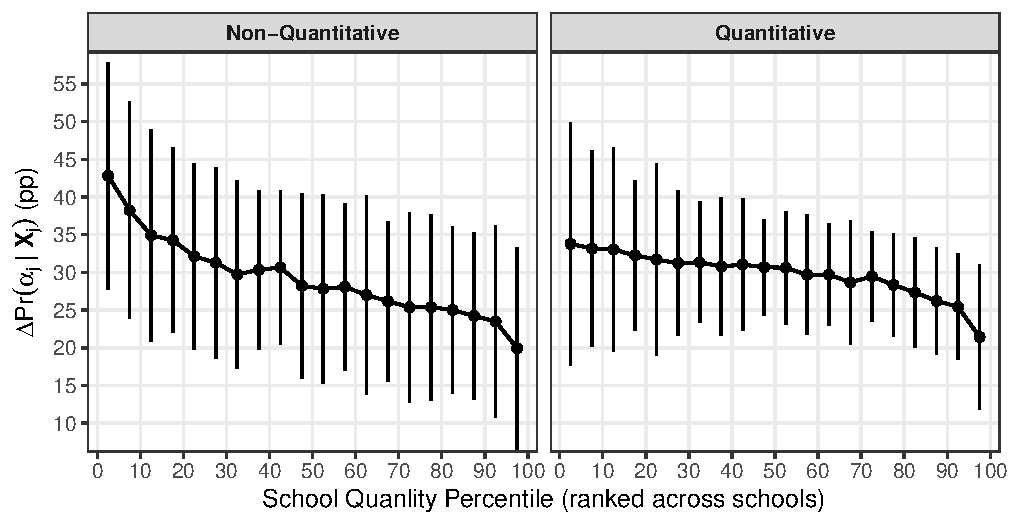
\includegraphics[width=\linewidth]
    {figures/Results/treatment_effects_by_schoolquality_subjectGroup_20.pdf}
    \label{fig:inflation_subject20}
  \end{subfigure}

  \vspace{-0.5em}
  
  \begin{subfigure}[t]{\linewidth}
    \centering
    \caption{2021}
    \vspace{-0.5em}
    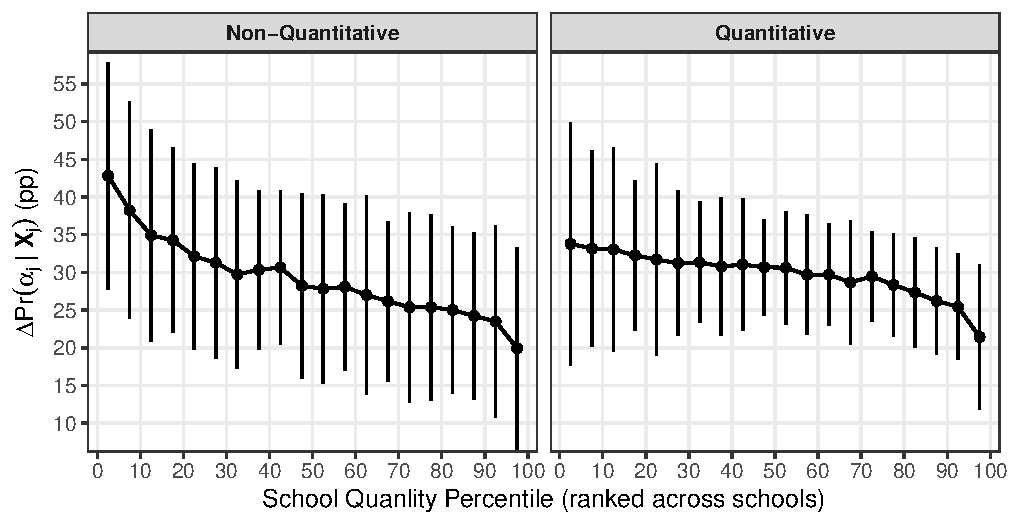
\includegraphics[width=\linewidth]{figures/Results/treatment_effects_by_schoolquality_subjectGroup_21.pdf}
    \label{fig:inflation_subject21}
  \end{subfigure}
  \label{fig:inflation_subjects_20_21}
  \vspace{-0.5em}
    \caption*{\footnotesize Note: This bin-scatter displays the subject group level increments in grade improvements defined as a student receiving a top grade (A or $\text{A}^*$) in (a) 2020 and (b) 2021. The sample is the universe of A-level exams used for admissions at British universities through the centralized administrative system (N = 2,802,651). Year-specific coefficients and 95\% confidence intervals are from a logistic regression that regresses a success dummy indicating the student receiving a top grade (A or $\text{A}^*$) on the interaction between school subject group dummy and a time indicator for both pandemic years. The regression controls for students' achievement score in a previous standardized national exam (GCSE) in mandatory subjects (mathematics and English literature) and a dummy variable for the subject course of the exam. Standard errors are clustered at the school-subject course level. }
\end{figure}
\clearpage

\begin{figure}[!htbp]
\label{fig:inflation_school_type}
  \caption{Grade inflation by school type}
  \vspace{-.5em}
  \centering
  \begin{subfigure}[t]{\linewidth}
    \centering
    \caption{}
    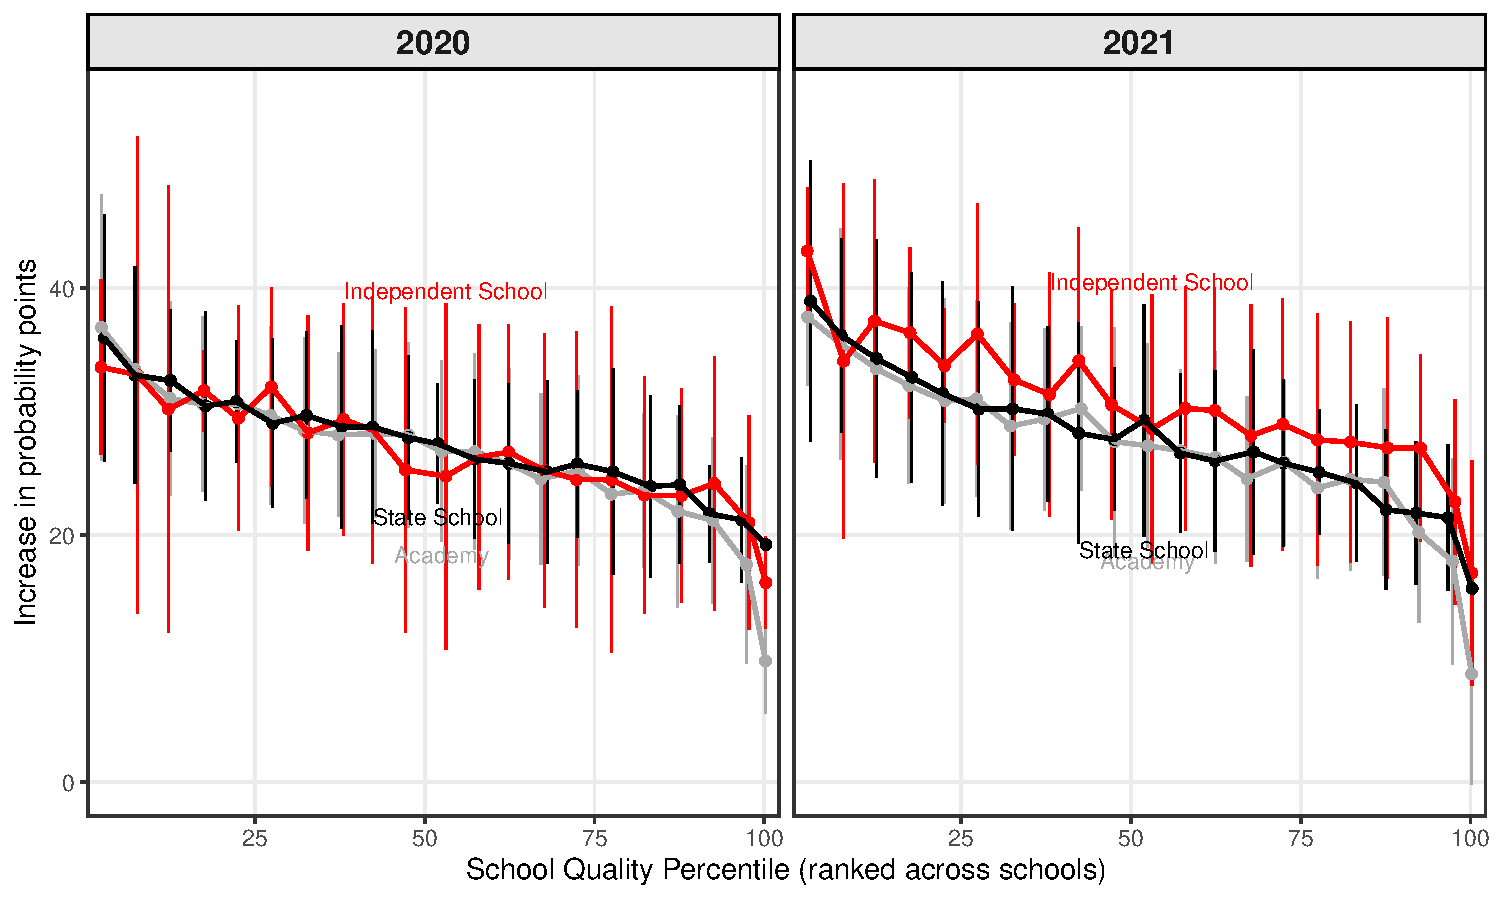
\includegraphics[width=.8\linewidth]{figures/Results/treatment_by_schooltype_indep.pdf}
    \label{fig:inflation_subject20}
  \end{subfigure}

  \vspace{4pt} % small gap between panels

  \begin{subfigure}[t]{\linewidth}
    \centering
    \caption{}
    \vspace{-.5em}
    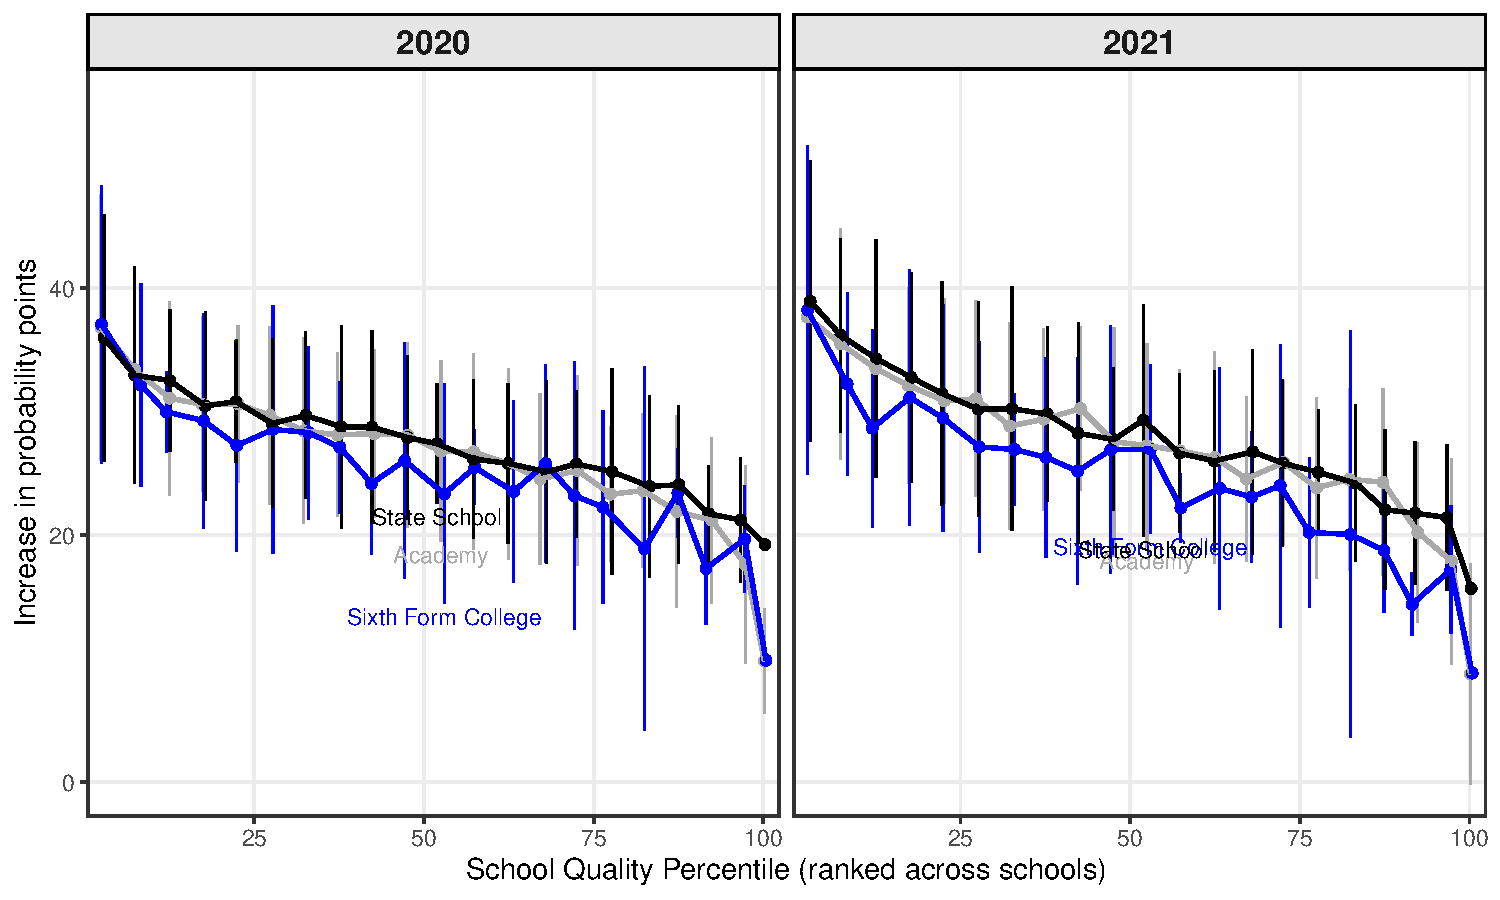
\includegraphics[width=.8\linewidth]{figures/Results/treatment_by_schooltype_sixth.pdf}
    \label{fig:inflation_subject21}
  \end{subfigure}
  \label{fig:inflation_subjects_20_21}
  \caption*{\footnotesize Note: The bin-scatter displays the school level increments in grade improvements defined as a student receiving a top grade (A or $\text{A}^*$) in (a) 2020 and (b) 2021. The sample is the universe of A-level exams used for admissions at British universities through the centralized administrative system (N = 2,802,651). Year-specific coefficients and 95\% confidence intervals are from a logistic regression that regresses a success dummy indicating the student receiving a top grade (A or $\text{A}^*$) on the interaction between school subject group dummy and a time indicator for both pandemic years. The regression controls for students' achievement score in a previous standardized national exam (GCSE) in mandatory subjects (mathematics and English literature) and a dummy variable for the subject course of the exam. Standard errors are clustered at the school-subject course level. }
\end{figure}
\clearpage

% in preamble: \usepackage{caption,subcaption}
\begin{figure}[!htb]
  \centering
    \caption{Aggregate dynamics}    
    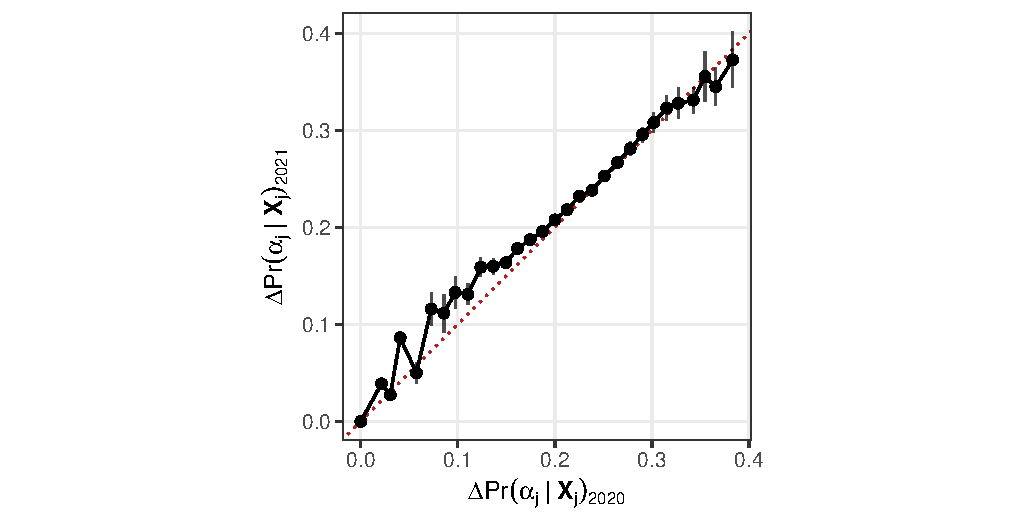
\includegraphics[width=1\linewidth]{figures/Results/DynamicsSchool_A.pdf}
    \label{fig:inflation_dynamics}
    \caption*{\footnotesize Note: The bin-scatter displays the school level grade improvements in 2021 relative the degree of grade improvements in 2020 for the same school. The sample is the universe of A-level exams used for admissions at British universities through the centralized administrative system (N = 2,802,651). Year-specific coefficients and 95\% confidence intervals are from a logistic regression that regresses a success dummy indicating the student receiving a top grade (A or $\text{A}^*$) on the interaction between school subject group dummy and a time indicator for both pandemic years. The regression controls for students' achievement score in a previous standardized national exam (GCSE) in mandatory subjects (mathematics and English literature) and a dummy variable for the subject course of the exam. Standard errors are clustered at the school-subject course level. }
\end{figure}

\begin{figure}
    \centering
    \caption{By subject groups}
    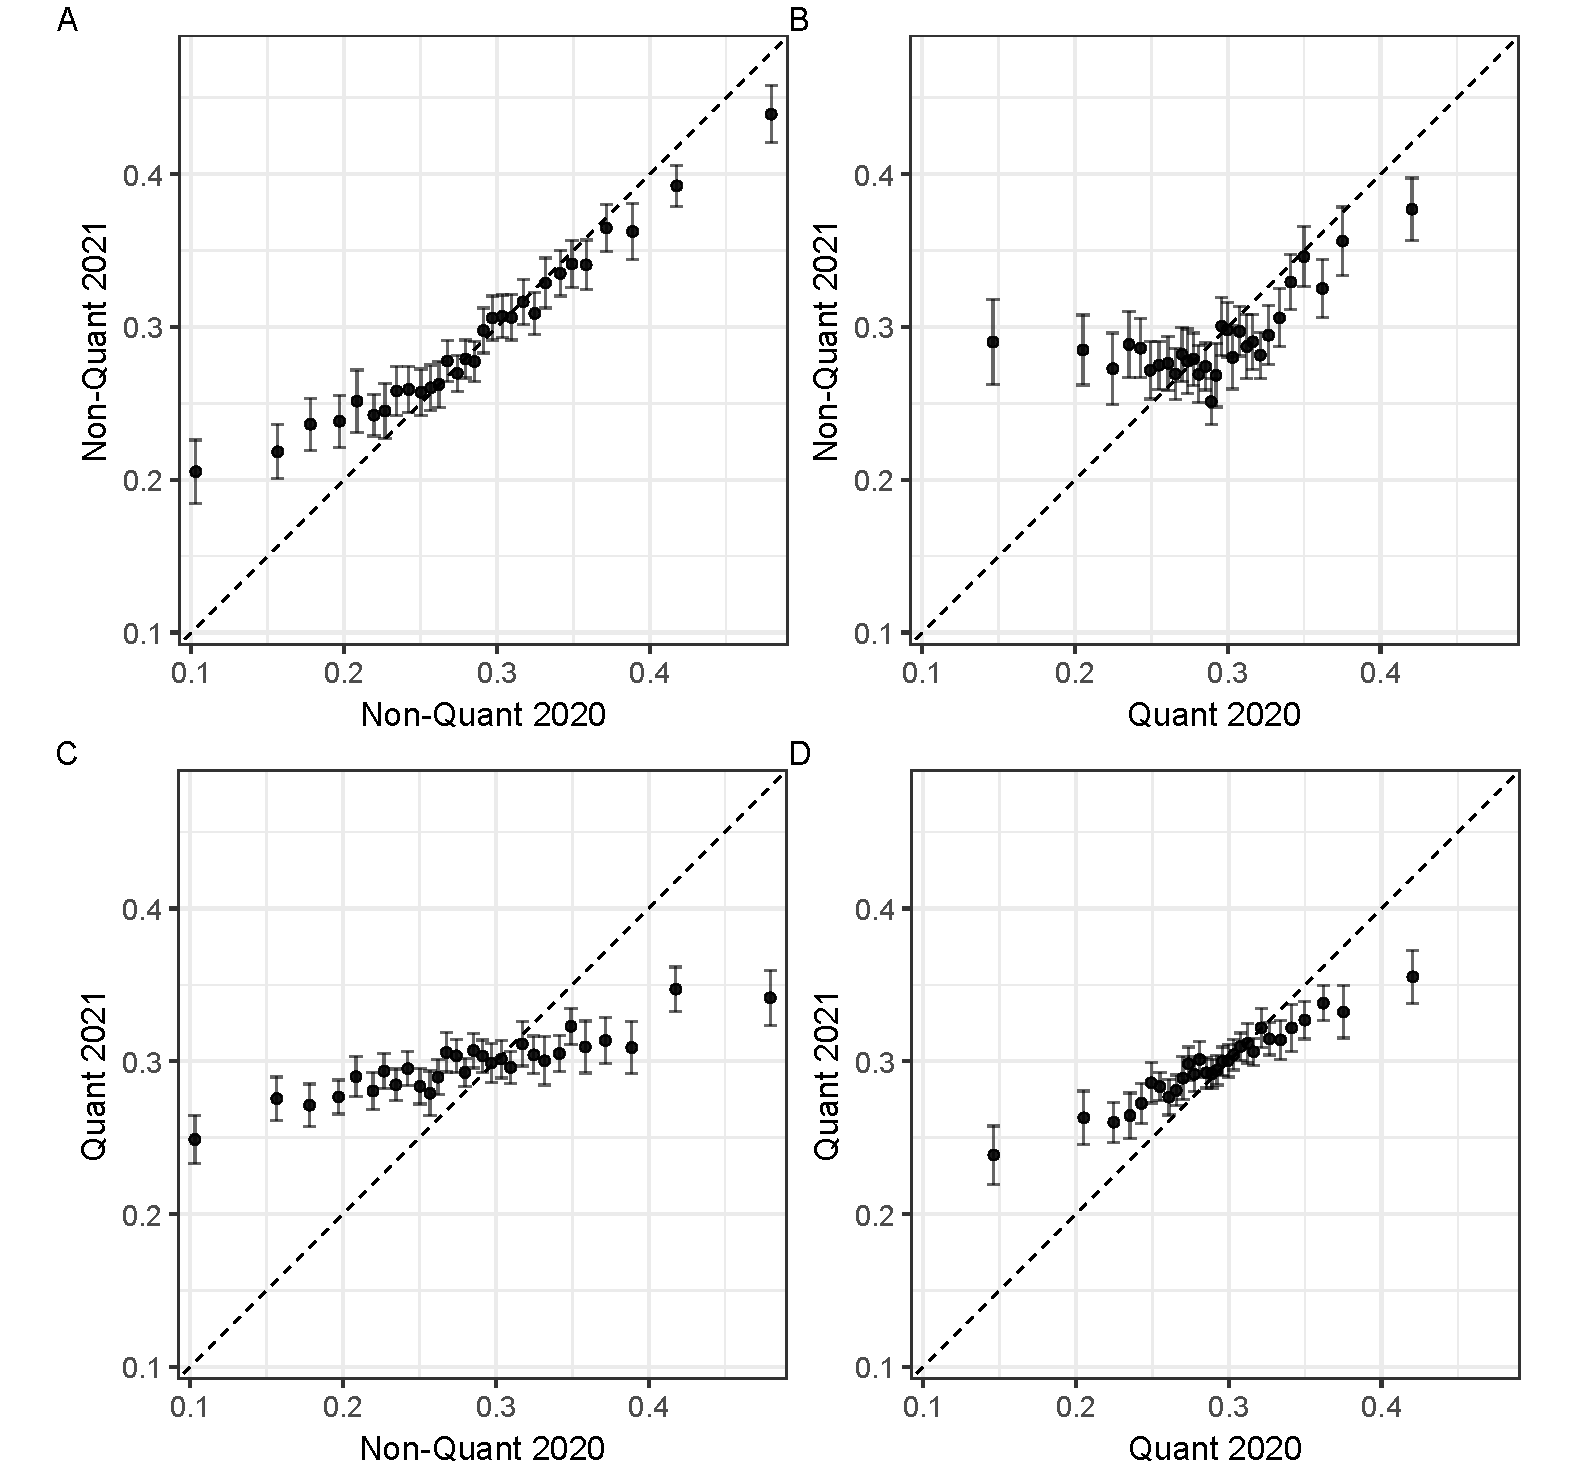
\includegraphics[width=\linewidth]{figures/Results/Dynamics_Course_2x2_rect_aligned.pdf}
    \label{fig:inflation_dynamics}
    \caption*{\footnotesize Note: The bin-scatter displays the school-subject-group level grade improvements in 2021 relative the degree of grade improvements in 2020 for the same school. The sample is the universe of A-level exams used for admissions at British universities through the centralized administrative system (N = 2,802,651). Year-specific coefficients and 95\% confidence intervals are from a logistic regression that regresses a success dummy indicating the student receiving a top grade (A or $\text{A}^*$) on the interaction between school subject group dummy and a time indicator for both pandemic years. The regression controls for students' achievement score in a previous standardized national exam (GCSE) in mandatory subjects (mathematics and English literature) and a dummy variable for the subject course of the exam. Standard errors are clustered at the school-subject course level. }
\end{figure}

\begin{figure}[!htbp]
  \centering
  \caption{Grade inflation by GCSE score by exam subject.}
  \begin{subfigure}[t]{\linewidth}
    \centering
    \caption{Gender gap in grade inflation by school quality}
    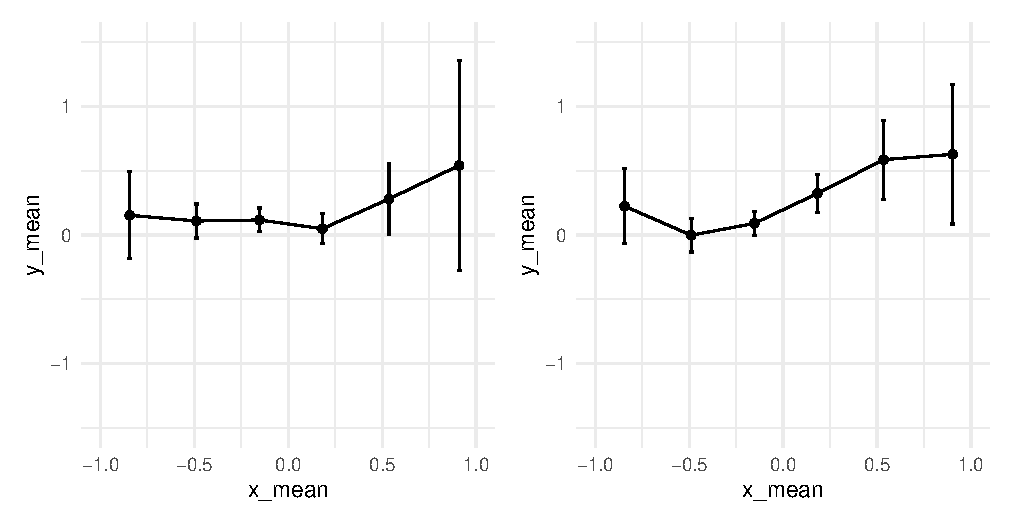
\includegraphics[width=0.94\linewidth]{figures/Results/Gender_BySchoolQuality_A.pdf}
    \label{fig:gender_sq}
  \end{subfigure}

  \vspace{0.8em}

  \begin{subfigure}[t]{\linewidth}
    \centering
    \caption{Ethnicity gap in grade inflation by school quality}
    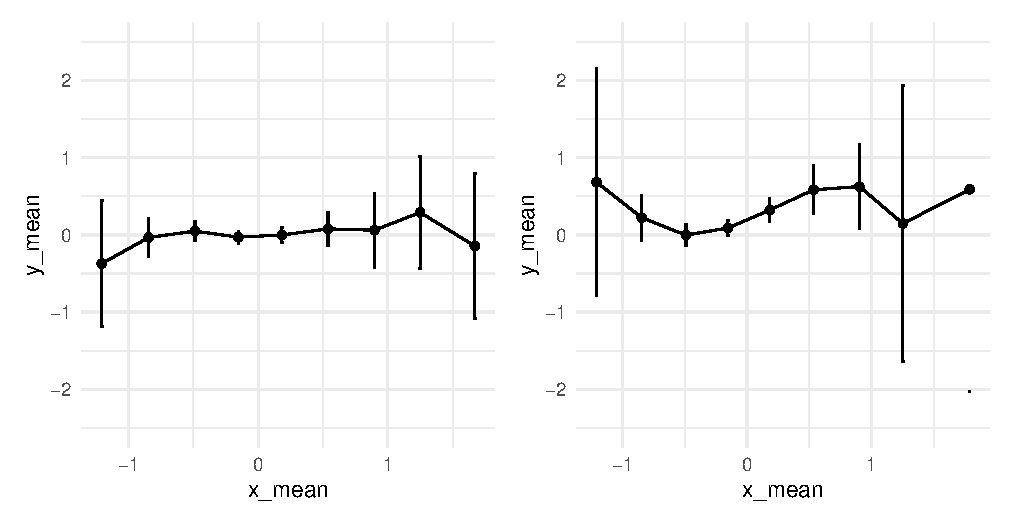
\includegraphics[width=0.94\linewidth]{figures/Results/Ethnic_BySchoolQuality_A.pdf}
    \label{fig:ethnic_sq}
  \end{subfigure}

  \label{fig:gender_ethnic_sq_combined}
  \caption*{\footnotesize Note: The bin-scatter displays the school level difference in grade improvements between (a)female and male students and (b) while and non-white students. The sample is the universe of A-level exams used for admissions at British universities through the centralized administrative system (N = 2,802,651). Year-specific coefficients and 95\% confidence intervals are from a logistic regression that regresses a success dummy indicating the student receiving a top grade (A or $\text{A}^*$) on the interaction between school subject group dummy and a time indicator for both pandemic years. The regression controls for students' achievement score in a previous standardized national exam (GCSE) in mandatory subjects (mathematics and English literature) and a dummy variable for the subject course of the exam. Standard errors are clustered at the school-subject course level. }
\end{figure}
\clearpage


\begin{figure}
    \centering
    \caption{Reduced form result of application success on grade inflation}
    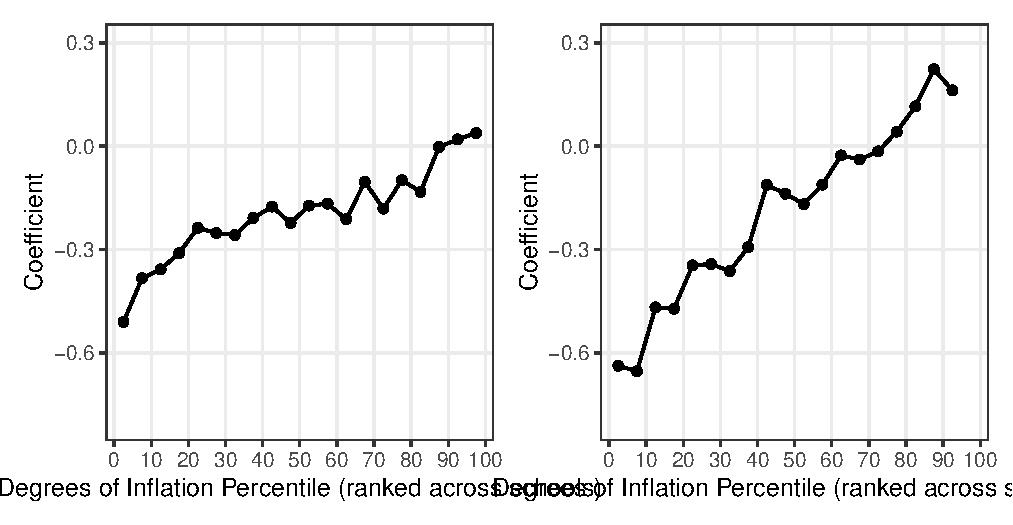
\includegraphics[width=\linewidth]{figures/Results/Reduced_Form.pdf}
    \label{fig:placeholder}
      \label{fig:gcse_combined}
  \caption*{\footnotesize Note: The figure displays school level improvements in success rate of securing a placement at a students top choice university program versus the extent of grade inflation at the school. The sample is the universe of A-level exams used for admissions at British universities through the centralized administrative system (N = 2,802,651). The y-axis coefficients and 95\% confidence intervals are from a student level logistic regression that regresses a success of student application on the interaction between school subject group dummy and a time indicator for both pandemic years. The x-axis coefficients and 95\% confidence intervals are from a student level logistic regression that regresses a dummy variable indicating whether a student received a top grade (A or $\text{A}^*$) in their exam on the interaction between school subject group dummy and a time indicator for both pandemic years. Both regressions control for students' achievement score in a previous standardized national exam (GCSE) in mandatory subjects (mathematics and English literature) and a dummy variable for the subject course of the exam. Standard errors are clustered at the school-subject course level. }
\end{figure}
\clearpage

\begin{figure}
    \centering
    \caption{Decomposition of university composition by source}
    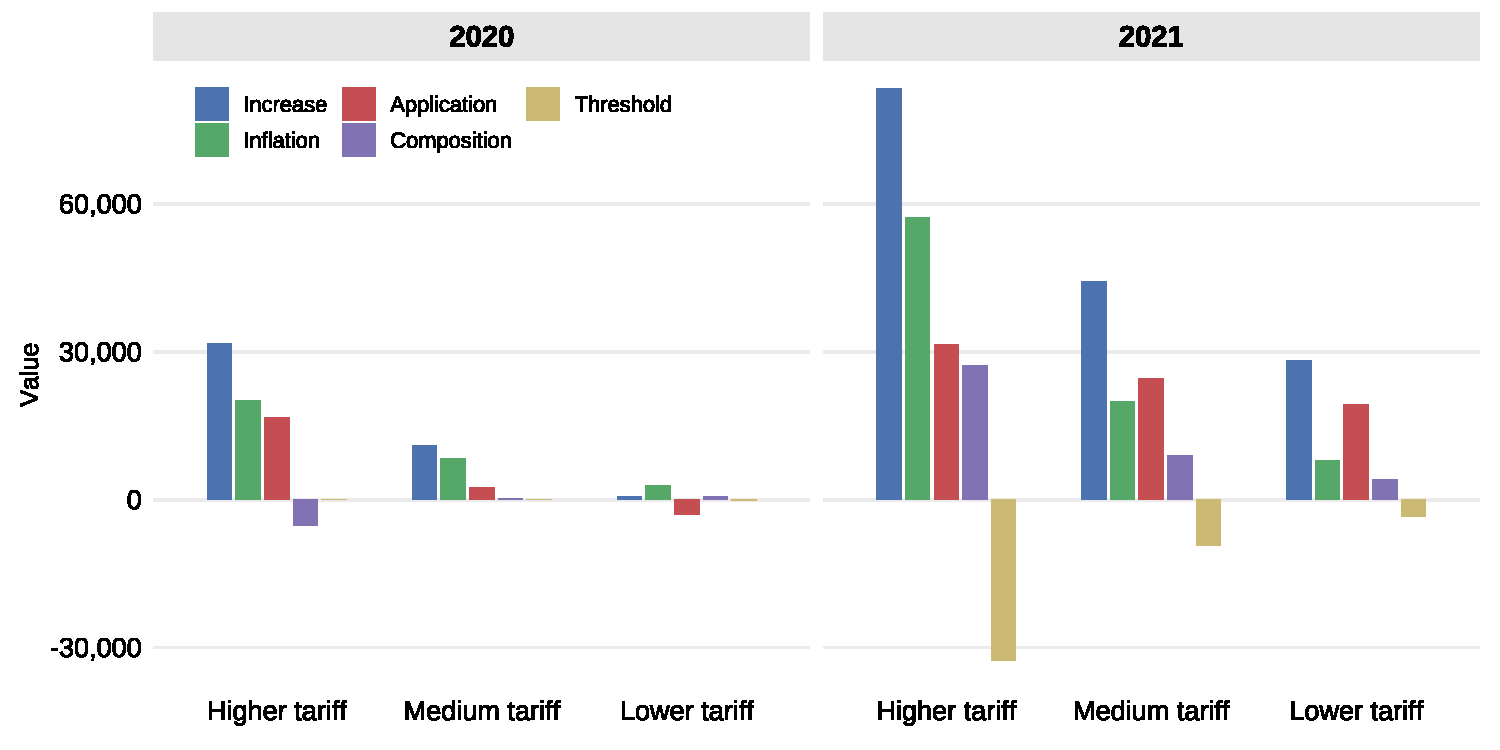
\includegraphics[width = \linewidth]{figures/Results/Aggregate.pdf}
    \label{fig:placeholder}
      \label{fig:gcse_combined}
      \caption*{\footnotesize Note: The bin plot displays a decomposition of the increase in the number of incoming student at each university tier group by separate channels. The sample is the universe of A-level exams used for admissions at British universities through the centralized administrative system (N = 2,802,651). Tariff groups denotes the degree of selectivity of the university program, with high tariff indicating the most selective university tier group and the lower tariff indicating the least selective group.}
\end{figure}
\clearpage


\clearpage